\documentclass{article}
\usepackage[francais]{babel}
\usepackage[utf8]{inputenc} % Required for including letters with accents
\usepackage[T1]{fontenc} % Use 8-bit encoding that has 256 glyphs
\usepackage{pythontex}
\usepackage{amsthm}
\usepackage{amsmath}
\usepackage{amssymb}
\usepackage{mathrsfs}
\usepackage{graphicx}
\usepackage{geometry}
\usepackage{stmaryrd}
\usepackage{tikz}
\usetikzlibrary{patterns}
%\usetikzlibrary{intersections}
\usepackage[cache=false]{minted}
\usepackage{xcolor}

\usepackage{stmaryrd}
%\usepackage{tikz}
%\usetikzlibrary{tikzmark}
\usepackage{empheq}
\usepackage{longtable}
\usepackage{booktabs} 
\usepackage{array}
\usepackage{pstricks}
\usepackage{pst-3dplot}
\usepackage{pst-tree}
\usepackage{pstricks-add}
\usepackage{upgreek}
%\usepackage{epstopdf}
\usepackage{eolgrab}
\usepackage{chngpage}
 \usepackage{calrsfs}
 % Appel du package pythontex 
\usepackage{pythontex}

\usepackage{algorithm2e}
\RestyleAlgo{algoruled}
  \SetKw{KwFrom}{from} 
\newenvironment{algo}{
\begin{algorithm}[H]
\DontPrintSemicolon \SetAlgoVlined}
{\end{algorithm}}



\usetikzlibrary{decorations.pathmorphing}
\def \de {{\rm d}}
\usepackage{color}
\usepackage{xcolor}
\newcommand{\mybox}[1]{\fbox{$\displaystyle#1$}}
\newcommand{\myredbox}[1]{\fcolorbox{red}{white}{$\displaystyle#1$}}
\newcommand{\mydoublebox}[1]{\fbox{\fbox{$\displaystyle#1$}}}
\newcommand{\myreddoublebox}[1]{\fcolorbox{red}{white}{\fcolorbox{red}{white}{$\displaystyle#1$}}}

\usepackage{xcolor}
%\setbeamercolor{background canvas}{bg=lightgray}
\definecolor{LightGray}{gray}{0.9}
\definecolor{monOrange}{rgb}{0.97,0.35,0.04}

 \title{Création de notre première application Vue}
\author{Ibrahim ALAME}
\date{14/02/2023}
\begin{document}
\maketitle

\section{La librairie create-vue}
\subsection{Première utilisation de la librairie {\color{monOrange} create-vue}}
Commencez par créer un dossier à l'emplacement que vous souhaitez. Ouvrez un terminal à l'emplacement du dossier et entrez la commande suivante :
\begin{minted}[
mathescape,
framesep=2mm,
baselinestretch=1.2,
fontsize=\footnotesize,
bgcolor=LightGray,
%linenos
]{bash}
npm init vue@latest
\end{minted}

Cette commande permet d'installer et d'exécuter la dernière version de {\color{monOrange}create-vue} qui permet de lancer la configuration d'une nouvelle application {\color{monOrange} Vue.js}. Lorsque vous entrez la commande pour la première fois vous aurez la demande de confirmation d'installer {\color{monOrange}create-vue }:
\begin{minted}[
mathescape,
framesep=2mm,
baselinestretch=1.2,
fontsize=\footnotesize,
bgcolor=LightGray,
%linenos
]{bash}
Need to install the following packages:
  create-vue@latest
Ok to proceed?
\end{minted}

Vous devrez simplement répondre {\tt y} ou {\tt yes}. Viennent ensuite toutes les questions sur la configuration de l'application. La première est le nom que vous souhaitez donner à votre application :
\begin{minted}[
mathescape,
framesep=2mm,
baselinestretch=1.2,
fontsize=\footnotesize,
bgcolor=LightGray,
%linenos
]{bash}
Project name: › vue-project
\end{minted}

Par défaut, le nom est prérempli avec vue-project mais vous pouvez bien sûr le changer.

La deuxième question est sur l'utilisation de TypeScript :
\begin{minted}[
mathescape,
framesep=2mm,
baselinestretch=1.2,
fontsize=\footnotesize,
bgcolor=LightGray,
%linenos
]{bash}
Add TypeScript? … No / Yes
\end{minted}
\begin{itemize}
\item Comme nous l'avons vu, choisissez {\color{blue} oui}.
\item Ensuite répondez {\color{blue} non} pour {\tt JSX}. Nous n'utiliserons pas {\tt JSX} qui est un langage de template React.
\item Répondez {\color{blue} non} pour {\tt Vue Router, Pinia, Vitest} et {\tt Cypress} car nous les verrons plus tard dans la formation.
\item Répondez {\color{blue} oui} à {\tt ESLint}, qui permet de contrôler la qualité du code et répondez oui à Prettier pour le formatage du code.
\end{itemize}


Vous devez en être là :
\begin{center}
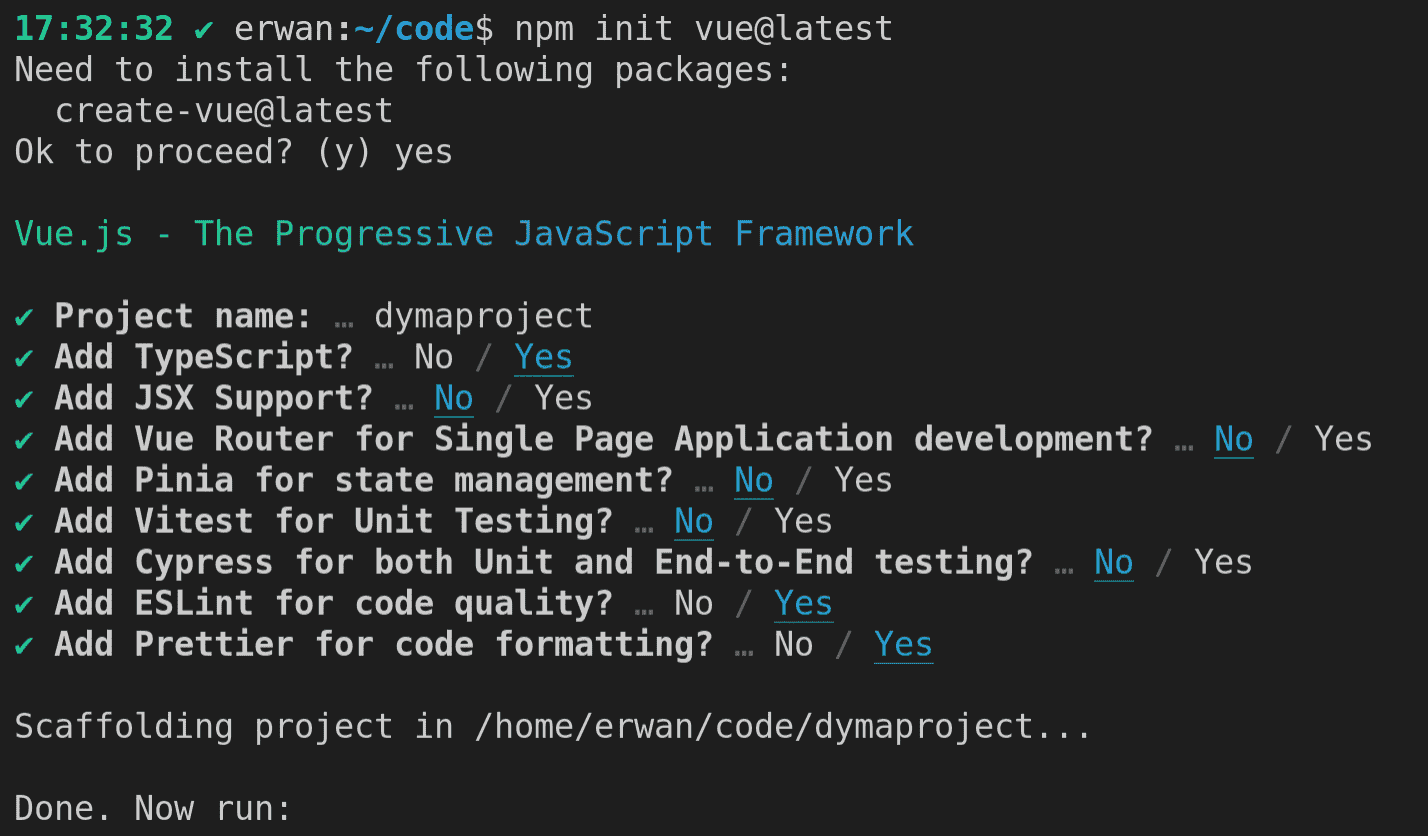
\includegraphics[width=10cm]{images/image04.png}
\end{center}

\subsection{Installation des dépendances}
Pour le moment, {\color{monOrange}create-vue} a déclaré toutes les dépendances et les configurations nécessaires en suivant vos options. Aucune dépendance {\tt JavaScript} n'a encore été installée par {\tt npm}. Pour les installer, il suffit d'ouvrir un terminal et d'aller dans le dossier de votre application, par exemple :
\begin{minted}[
mathescape,
framesep=2mm,
baselinestretch=1.2,
fontsize=\footnotesize,
bgcolor=LightGray,
%linenos
]{bash}
cd dymaproject
\end{minted}

Et ensuite de lancer l'installation des dépendances :
\begin{minted}[
mathescape,
framesep=2mm,
baselinestretch=1.2,
fontsize=\footnotesize,
bgcolor=LightGray,
%linenos
]{bash}
npm install
\end{minted}

\subsection{Utilisation du linter}
Un linter est un outil d'analyse de code qui permet de détecter les erreurs et les problèmes de syntaxe. La configuration du linter, en l'occurrence {\tt ESLint} est dans le fichier {\tt .eslintrc.cjs} :
\begin{minted}[
mathescape,
framesep=2mm,
baselinestretch=1.2,
fontsize=\footnotesize,
bgcolor=LightGray,
%linenos
]{javascript}
/* eslint-env node */
require('@rushstack/eslint-patch/modern-module-resolution')

module.exports = {
  root: true,
  'extends': [
    'plugin:vue/vue3-essential',
    'eslint:recommended',
    '@vue/eslint-config-typescript',
    '@vue/eslint-config-prettier/skip-formatting'
  ],
  parserOptions: {
    ecmaVersion: 'latest'
  }
}
\end{minted}

{\color{monOrange} create-vue} a donc automatiquement créé la bonne configuration du linter pour une utilisation avec {\tt Vue.js}. Pour exécuter le linter avec la configuration faites :

\begin{minted}[
mathescape,
framesep=2mm,
baselinestretch=1.2,
fontsize=\footnotesize,
bgcolor=LightGray,
%linenos
]{bash}
npm run lint
\end{minted}     

Cela exécutera le script {\tt lint} déclaré dans le fichier {\tt package.json}. Pour l'instant il y a bien sûr aucune indication car nous n'avons pas commencé à coder ! Mais exécuter cette commande de temps en temps lors du développement permet d'éviter certaines erreurs et de suivre les recommandations pour les bonnes pratiques en matière de syntaxe (appelées coding style).

\subsection{Lancer le serveur de développement}
Pour lancer le serveur de développement il suffit d'exécuter le script dev :
\begin{minted}[
mathescape,
framesep=2mm,
baselinestretch=1.2,
fontsize=\footnotesize,
bgcolor=LightGray,
%linenos
]{bash}
npm run dev
\end{minted} 

Cela va en fait exécuter {\color{monOrange}vite} qui va lancer son serveur de développement. Vous pourrez ainsi accéder à l'application {\tt Vue.js} dans votre navigateur à l'adresse {\color{monOrange} http://localhost:5173/}.

%%%%%%%%%%%%%%%%%%%%%%%%%%%%%%%%%%%%%%%%%%%%%%%%%%%%%%%%%%%%%%%%%
\section{Architecture initiale}
\subsection{Architecture initiale d'un projet généré par create-vue}
L'architecture initiale du projet généré est la suivante :
\begin{center}
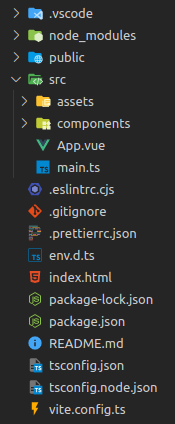
\includegraphics[width=3cm]{images/image05.png}
\end{center}

\subsection{Détail des fichiers et des dossiers}
\begin{itemize}
\item {\tt vite.config.js} : fichier de configuration de Vite.
\item {\tt tsconfig.node.json} : fichier de configuration de Vite pour pouvoir utiliser TypeScript. Vous pouvez retirer vitest, cypress, playwright de la propriété types car nous ne les utiliserons pas pour le moment :


\begin{minted}[
mathescape,
framesep=2mm,
baselinestretch=1.2,
fontsize=\footnotesize,
bgcolor=LightGray,
%linenos
]{javascript}
{
  "extends": "@vue/tsconfig/tsconfig.node.json",
  "include": ["vite.config.*"],
  "compilerOptions": {
    "composite": true,
    "types": ["node"]
  }
}
\end{minted} 
\item {\tt tsconfig.json} : fichier de configuration de TypeScript. Toutes les applications utilisant TypeScript ont ce fichier. Il permet de configurer notamment les options pour transpiler le TypeScript en JavaScript.
\item {\tt README.md} : décrit brièvement les différentes commandes possibles et la configuration recommandée de l'éditeur VS Code.
\item {\tt package.json} et {\tt package-lock.json} : ces fichiers {\tt JSON} permettent de décrire le projet et surtout de détailler les dépendances et leurs versions requises pour l'utiliser. Il décrit également les scripts pouvant être lancés avec {\color{monOrange}npm run}.
\end{itemize}
Les scripts disponibles sont :
\begin{itemize}
\item {\color{blue} dev} : qui permet de lancer le serveur de développement de {\color{monOrange} Vite} en local.
\item  {\color{blue} build} : qui permet de construire la version de l'application optimisée pour la production.
\item  {\color{blue} preview}  : qui permet de visualiser la version de production en local (par exemple avant de la mettre réellement en production sur des serveurs).
\item  {\color{blue} typecheck}  : qui permet de vérifier les types du code {\color{monOrange} TypeScript} sans transpiler le {\color{monOrange} TypeScript} en {\tt JavaScript}.
\item  {\color{blue} lint}  : qui permet d'exécuter {\color{monOrange} ESLint} avec les bonnes options.
\item  {\color{blue} index.html } : template {\tt HTML} qui sera envoyé au navigateur.
\item  {\color{blue} env.d.ts}  : fichier qui permet de charger des types supplémentaires pour utiliser {\color{monOrange} TypeScript} avec {\color{monOrange} Vue.js}.
\item  {\color{blue} .gitignore}  : permet de lister les fichiers qui ne doivent pas être pris en compte par {\color{monOrange} Git}.

\item  {\color{blue} .eslintrc}  : fichier de configuration de {\color{monOrange} ESLint} que nous avons déjà expliqué.
\item  {\color{blue} src } : dossier qui contient les fichiers sources de votre application (d'où le nom {\color{monOrange} src} pour source).
\item  {\color{blue} public}  : dossier qui contient les fichiers qui n'ont pas besoin d'être traité par {\color{monOrange} Vite} ou par aucun outil et qui sont directement envoyés par le serveur au navigateur.
\item  {\color{blue} src/main.ts}  : il s'agit du point d'entrée de notre application. Nous expliquerons plus loin dans le cours la fonction {\tt createApp()} ainsi que {\tt \$mount}. Sachez simplement que nous importons notre composant racine {\color{monOrange} App} et créons l'instance racine de l'application ici.
\item  {\color{blue} src/App.vue}  : il s'agit du composant référencé dans {\color{monOrange} main.ts} qui constitue la racine des vues de notre application. Il s'agit du premier composant rendu, et de lui découle les rendus de tous les autres composants. Nous étudierons la structure des composants dans une prochaine leçon.
\item  {\color{blue} src/components}  : dossier qui contient les composants de notre application {\color{monOrange} Vue}.
\item  {\color{blue} src/components/HelloWorld.vue}  : sous-composant de {\color{monOrange} App.vue}.
\item  {\color{blue} src/assets}  : dossier contenant les ressources de l'application comme les images, le {\tt CSS} etc.
\item  {\color{blue} node\_modules}  : contient toutes les dépendances installées par {\color{monOrange} npm}.
\end{itemize}

%%%%%%%%%%%%%%%%%%%%%%%%%%%%%%%%%%%%%%%%%%%%%%%%%%%%%%%%%%%%%%%%%%%%%%%%%


\section{Comment fonctionne Vue ?}
Nous allons voir les fichiers par ordre logique. Le navigateur reçoit en premier l'{\color{monOrange}index.html}.

\subsection{Le fichier {\color{monOrange}index.html}}
Le fichier index.html est ce que le navigateur va lire en premier :
\begin{minted}[
mathescape,
framesep=2mm,
baselinestretch=1.2,
fontsize=\footnotesize,
bgcolor=LightGray,
%linenos
]{html}
<!DOCTYPE html>
<html lang="en">
  <head>
    <meta charset="UTF-8" />
    <link rel="icon" href="/favicon.ico" />
    <meta name="viewport" content="width=device-width, initial-scale=1.0" />
    <title>Vite App</title>
  </head>
  <body>
    <div id="app"></div>
    <script type="module" src="/src/main.ts"></script>
  </body>
</html>
\end{minted} 

Notez bien qu'il y a une {\tt div} conteneur avec l'{\color{monOrange}id app}. Notez également que le fichier src/main.ts est chargé comme un module {\tt JavaScript}. Le navigateur demande donc ce module au serveur.

\subsection{Le fichier {\color{monOrange}src/main.ts}}
Le fichier {\color{monOrange}main.ts} est le point d'entrée de l'application car c'est le premier fichier {\tt JavaScript} chargé par le navigateur.

Note : le fichier est en {\color{monOrange}.ts} car c'est un fichier {\tt TypeScript} mais il sera transpilé par Vite en {\tt JavaScript} que ce soit pour le développement ou la production. En effet, le navigateur ne comprend que le langage {\tt JavaScript} et pas le {\tt TypeScript}.
\begin{minted}[
mathescape,
framesep=2mm,
baselinestretch=1.2,
fontsize=\footnotesize,
bgcolor=LightGray,
%linenos
]{javascript}
import { createApp } from "vue";
import App from "./App.vue";

createApp(App).mount("#app");
\end{minted} 

{\tt import App from "./App.vue";} permet d'importer le composant {\color{monOrange}App} que nous verrons juste après. {\tt createApp()} permet de créer une instance de votre application {\color{monOrange}Vue.js}. Elle prend en argument, le composant racine, c'est-à-dire le premier composant de votre application qui aura d'autres composants enfants.

{\tt mount()} permet de monter l'application instanciée par {\tt createApp()} dans un conteneur qui est identifié par un sélecteur {\tt CSS}. Ici, cela signifie que le composant racine {\color{monOrange}App} sera monté sur le conteneur dont l'{\color{monOrange}id} est {\color{monOrange}app} :
\begin{minted}[
mathescape,
framesep=2mm,
baselinestretch=1.2,
fontsize=\footnotesize,
bgcolor=LightGray,
%linenos
]{html}
<div id="app"></div>
\end{minted} 

Le composant sera ainsi affiché (on dit plus souvent rendu) dans ce conteneur.

\subsection{Le fichier {\color{monOrange}src/App.vue}}
Le fichier {\tt App.vue} est le composant racine. C'est le premier composant de l'application qui est chargé et instancié par {\tt createApp()}. Ce composant est le sommet de ce qu'on appelle l'arbre des composants : à savoir l'organisation hiérarchique des composants de l'application. Une application a des dizaines voir des centaines de composants qui sont organisés en arbre à partir du composant racine :
\begin{center}
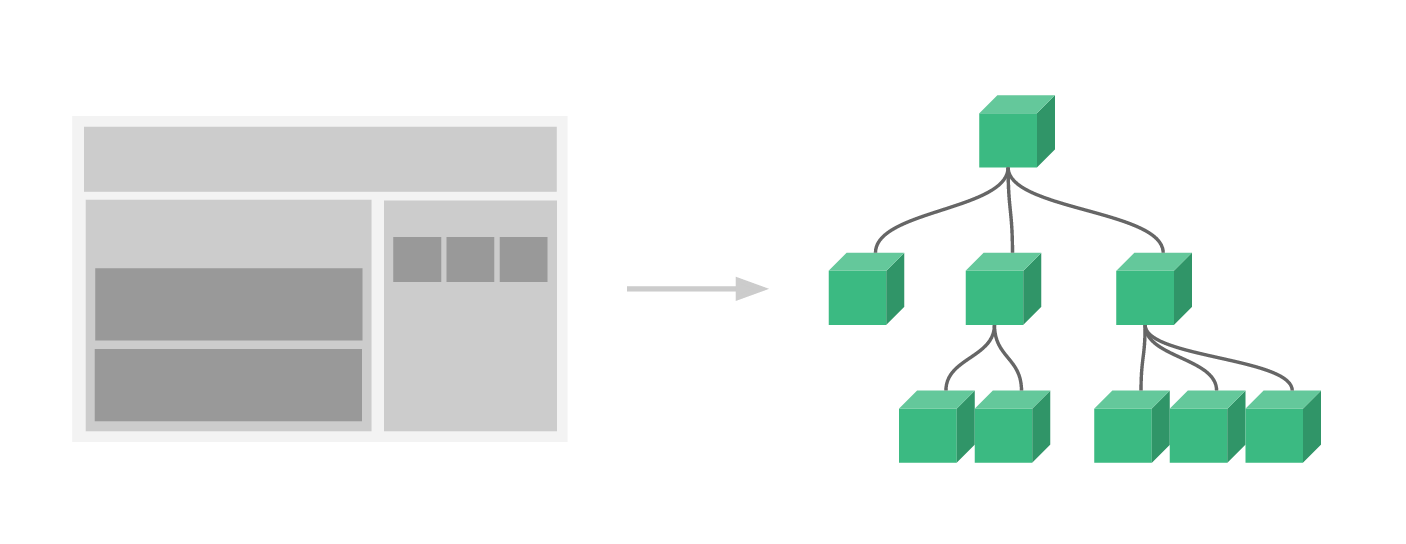
\includegraphics[width=12cm]{images/image06.png}
\end{center}

Remarquez déjà que le composant {\color{monOrange}App.vue} est constitué de trois parties : {\tt template, script} et {\tt style}. Nous étudierons bientôt les composants en détail.

\subsection{Aller plus loin sur le fonctionnement de Vue.js : le {\color{monOrange}DOM virtuel}}
Nous allons d'abord effectuer quelques rappels avant d'approfondir le fonctionnement de Vue.js.
\subsubsection{Le DOM (Document Object Model)}
Le {\tt DOM} permet de passer du {\tt HTML} à un grand objet document qui est un arbre regroupant tous les éléments déclarés en {\tt HTML}. Autrement dit, lorsque le navigateur reçoit le {\tt HTML} de la page, il va le parser (c'est-à-dire l'analyser) et le transformer en {\tt DOM} grâce à des algorithmes. Ainsi, les attributs {\tt HTML} deviennent automatiquement des propriétés des objets du {\tt DOM}. Par exemple :
\begin{minted}[
mathescape,
framesep=2mm,
baselinestretch=1.2,
fontsize=\footnotesize,
bgcolor=LightGray,
%linenos
]{html}
<body id="page">
\end{minted} 

Devient un nœud sur l'objet document qui sera un objet body contenant une propriété id contenant la valeur page.

Il existe plusieurs types de noeuds :
\begin{center}
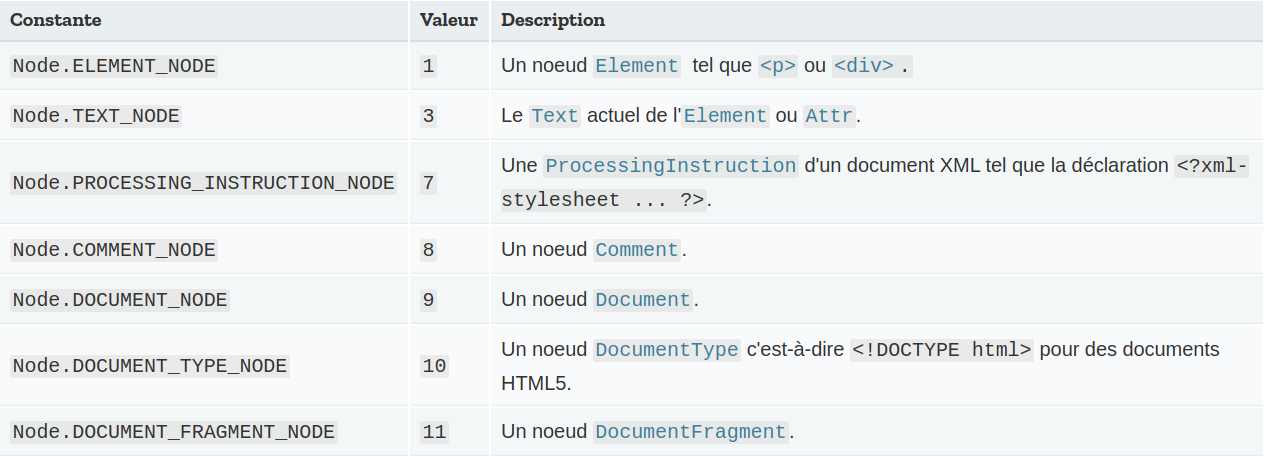
\includegraphics[width=15cm]{images/image07.png}
\end{center}

\subsubsection{Le DOM virtuel}
Dans les applications Web modernes, il peut y avoir des centaines ou des milliers de nœuds sur lesquels sont enregistrés de nombreux gestionnaires d'événements. En conséquence, de très nombreuses mises à jour du {\tt DOM} doivent être réalisées. Or, ces mises à jour sont très coûteuses en performance car plus le {\tt DOM} est grand, plus les recherches et les changements sont coûteux. {\color{monOrange}Vue.js} utilise donc un {\tt DOM} virtuel (appelé {\tt VDOM}) qui est une représentation du {\tt DOM} en {\tt JavaScript}. Le {\tt DOM } virtuel n'est donc qu'un simple, immense, objet {\tt JavaScript} :
\begin{minted}[
mathescape,
framesep=2mm,
baselinestretch=1.2,
fontsize=\footnotesize,
bgcolor=LightGray,
%linenos
]{javascript}
const vnode = {
  type: 'div',
  props: {
    id: 'hello'
  },
  children: [
    /* plein de vnodes */
  ]
}
\end{minted} 

Les noeuds du DOM virtuels sont appelés des noeuds virtuels ou {\color{monOrange}vnode} (pour virtual node). {\color{monOrange}Vue.js} va transformer le {\tt VDOM} en {\tt DOM} pour que le navigateur puisse afficher la page. Ce processus est appelé le montage (mount en anglais).

Lorsque des mises à jour sur la page doivent intervenir, le {\tt DOM} virtuel est modifié avant que les modifications sur le {\tt DOM} ne soient effectuées. Le {\tt DOM} virtuel est une représentation légère du {\tt DOM} en {\tt JavaScript} qui peut être utilisée par des algorithmes très performants de comparaison des différences entre {\tt DOM} virtuel et {\tt DOM}.

Dès lors que le {\tt DOM} doit être modifié, un patch est appliqué par {\color{monOrange}Vue.js} de manière extrêmement optimisée pour ne réaliser que les changements absolument nécessaires. Par exemple, si aucune valeur affichée ne change, alors aucune mise à jour du {\tt DOM} n'est déclenchée ce qui économise beaucoup en performance.

En résumé, {\color{monOrange}Vue.js} va créer au départ un {\tt DOM} virtuel puis le convertir en {\tt DOM HTML} pour l'affichage lors du montage. Lorsque des changements interviennent, par exemple un événement survient, les changements affectant le {\tt DOM} virtuel sont analysés par des algorithmes et seuls les changements ayant un effet sur l'affichage sont propagés au {\tt DOM} lors de la phase de mise à jour (patch ou diffing en anglais). Ainsi, seules les insertions, les modifications et les suppressions d'éléments {\tt HTML} absolument nécessaires sont effectuées, ce qui permet un énorme gain de performance.

%%%%%%%%%%%%%%%%%%%%%%%%%%%%%%%%%%%%%%%%%%%%%%%%%%%%%%%%%%%

\section{Les API composition et options}
{\color{monOrange}Vue.js} propose deux API pour écrire des composants {\color{monOrange}Vue} : l'API options et l'API composition.
\begin{itemize}
\item L'API options est l'API originelle qui existe depuis la première version du {\color{monOrange}framework}.
\item L'API composition est l'API avec laquelle {\color{monOrange}Vue} a été réécrite pour la version 3. C'est la nouvelle API qui est aujourd'hui recommandée et celle que nous verrons dans la formation.
\end{itemize}
\subsection{L'API options}
Dans l'ancienne API options, la logique du composant est définie dans un objet comportant des options comme {\tt data}, {\tt methods} ou {\tt mounted} par exemple. Les propriétés sont définies sur l'objet {\tt this} disponible dans les options.

Nous ne détaillerons pas plus car ce n'est pas l'API que nous utiliserons. Nous la présentons uniquement pour que vous puissiez la reconnaître lorsque vous la rencontrez. Voici à quoi ressemble un composant écrit avec l'API options :
\begin{minted}[
mathescape,
framesep=2mm,
baselinestretch=1.2,
fontsize=\footnotesize,
bgcolor=LightGray,
%linenos
]{html}
<script>
export default {
  data() {
    return {
      count: 0
    }
  },
  methods: {
    increment() {
      this.count++
    }
  },
  mounted() {
    console.log(`La valeur initiale est ${this.count}.`)
  }
}
</script>

<template>
  <button @click="increment">Valeur du compteur : {{ count }}</button>
</template>
\end{minted} 

\subsection{L'API composition}
Avec l'API composition nous définissons la logique d'un composant en important des fonctions. Voilà le même exemple avec la nouvelle API :
\begin{minted}[
mathescape,
framesep=2mm,
baselinestretch=1.2,
fontsize=\footnotesize,
bgcolor=LightGray,
%linenos
]{html}
<script setup>
import { ref, onMounted } from 'vue'

const count = ref(0)
function increment() {
  count.value++
}

onMounted(() => {
  console.log(`La valeur initiale est ${count.value}.`)
})
</script>

<template>
  <button @click="increment">Valeur du compteur : {{ count }}</button>
</template>
\end{minted} 

\subsection{Les {\color{monOrange}Single-File Components} (SFC)}
Les SFC sont des composants écrits dans des fichiers qui terminent par l'extension {\color{monOrange}.vue}. Un SFC comporte la logique du composant (partie script en {\tt JavaScript/TypeScript}), le template (en {\tt HTML}) et le style (en {\tt CSS} ou {\tt Sass}).

Il est fortement recommandé d'utiliser les SFC pour écrire des composants {\color{monOrange}Vue.js}. C'est d'ailleurs ce que nous utiliserons tout le long de la formation.

%%%%%%%%%%%%%%%%%%%%%%%%%%%%%%%%%%%%%%%%%%%%%%%%%%%%%%%

\section{Création d'un composant}
\subsection{Passer en mode {\color{monOrange}Take Over}}
L'extension {\color{monOrange}Volar} est plus performante pour gérer l'utilisation de {\tt TypeScript} avec {\color{monOrange}Vue.js}. Aussi, il faut configurer l'éditeur {\tt VS Code} pour lui dire que nous utilisons {\color{monOrange}Volar}.

Pour ce faire, aller sur l'onglet {\tt Extensions de VS Code}. Recherchez {\tt @builtin typescript}. Cliquez sur {\tt TypeScript and JavaScript Language Features}. Cliquez sur {\tt Désactiver (espace de travail)}. Cela désactivera uniquement pour ce projet. Cliquez ensuite sur Rechargement requis.

\subsection{Utilisation du mode {\color{monOrange}strict} de {\color{monOrange}TypeScript}}
Pour activer l'option {\color{monOrange}strict} du compilateur {\tt TypeScript} modifiez le fichier {\tt tsconfig.json} :
\begin{minted}[
mathescape,
framesep=2mm,
baselinestretch=1.2,
fontsize=\footnotesize,
bgcolor=LightGray,
%linenos
]{javascript}
{
  "extends": "@vue/tsconfig/tsconfig.web.json",
  "include": ["env.d.ts", "src/**/*", "src/**/*.vue"],
  "compilerOptions": {
    "strict": true,
    "baseUrl": ".",
    "paths": {
      "@/*": ["./src/*"]
    }
  },
  "references": [
    {
      "path": "./tsconfig.node.json"
    }
  ]
}
\end{minted} 

Cette option permet d'activer de nombreuses configurations plus strictes pour le contrôle des types par le compilateur. Cela permet d'améliorer sa capacité à détecter des erreurs.

\subsection{Création du premier composant}
Commençons par supprimer les composants mis en place automatiquement par {\color{monOrange}create-vue} pour la page de présentation lors du lancement de l'application. 
\begin{enumerate}
\item Supprimez tous les fichiers et les dossiers dans {\tt src/components/}.
\item Supprimez le contenu, mais pas le fichier de {\tt src/App.vue}.
\end{enumerate}

Comme nous l'avons vu, un composant {\color{blue} monofichier} (SFC, pour Single-file component) est un fichier {\color{blue} .vue} dont le nom est par convention en {\tt PascalCase}. Un composant monofichier a donc un template qui comporte le {\tt HTML}, une partie script qui comporte le JavaScript et une partie style qui comporte le {\tt CSS}. Voici l'exemple minimal de la vidéo :
\begin{minted}[
mathescape,
framesep=2mm,
baselinestretch=1.2,
fontsize=\footnotesize,
bgcolor=LightGray,
%linenos
]{html}
<template>
    <h1>Bonjour {{name}}</h1>
</template>

<script setup lang="ts">
    const name = 'Jean';
</script>

<style></style>
\end{minted} 

%\subsection{Exemple exécutable}
%Vous pouvez aussi directement utiliser ce code exécutable. N'hésitez pas à l'ouvrir dans un nouvel onglet :

%%%%%%%%%%%%%%%%%%%%%%%%%%%%%%%%%%%%%%%%%%%%%%%%%%%%%%

\section{Vue.js sans Vite}
\subsection{Utiliser {\color{monOrange}Vue.js} sans {\color{monOrange}Vite}}
Créez un dossier projet-vue.

Dans ce dossier, créez un fichier index.html :
\begin{minted}[
mathescape,
framesep=2mm,
baselinestretch=1.2,
fontsize=\footnotesize,
bgcolor=LightGray,
%linenos
]{html}
<!DOCTYPE html>
<html lang="en">
  <head>
    <meta charset="UTF-8" />
    <meta http-equiv="X-UA-Compatible" content="IE=edge" />
    <meta name="viewport" content="width=device-width, initial-scale=1.0" />
    <title>Document</title>
    <script src="https://unpkg.com/vue@3"></script>
  </head>
  <body>
    <div id="app">
      <h1>Bonjour {{ name }}</h1>
    </div>

    <script>
      Vue.createApp({
        setup() {
          const name = 'test';
          return {
            name,
          };
        },
      }).mount('#app');
    </script>
  </body>
</html>
\end{minted} 

Ici, nous n'utilisons que la librairie {\color{monOrange}Vue.js} sans {\color{monOrange}Vite} et sans aucune autre librairie. 
\begin{itemize}
\item Il n'y a aucune étape de {\tt build}, nous ne pouvons pas utiliser Sass, TypeScript etc.

\item Il n'y a pas de minification du code et pleins d'avantages apportés par {\color{monOrange}Vite}.
\end{itemize}
Cet exemple permet simplement de montrer comment utiliser {\color{monOrange}Vue.js} seul mais dans toute la formation nous n'utiliserons pas du tout cette méthode car il est impossible d'écrire une application complexe comme cela. Cette manière de faire peut être utile pour par exemple gérer une barre de recherche sur une application avec {\color{monOrange}Symfony} côté serveur.




\end{document}

